\section{Interpolazione}\label{cap:interpolazione}

Come accennato nel capitolo \ref{cap:parametri}, la frequenza di campionamento e il numero di campioni estratti per frame non garantiscono la precisione desiderata.
La soluzione introdotta per aumentare tale precisione è interpolare i valori attorno al massimo trovato.
L'interpolazione utilizzata è di tipo \emph{spline}.
Sono stati interpolati ventuno punti, dieci con ascissa inferiore a quella del massimo, il massimo stesso e dieci con ascissa superiore al massimo.

	\begin{figure}[h]
	  \begin{center} 
	    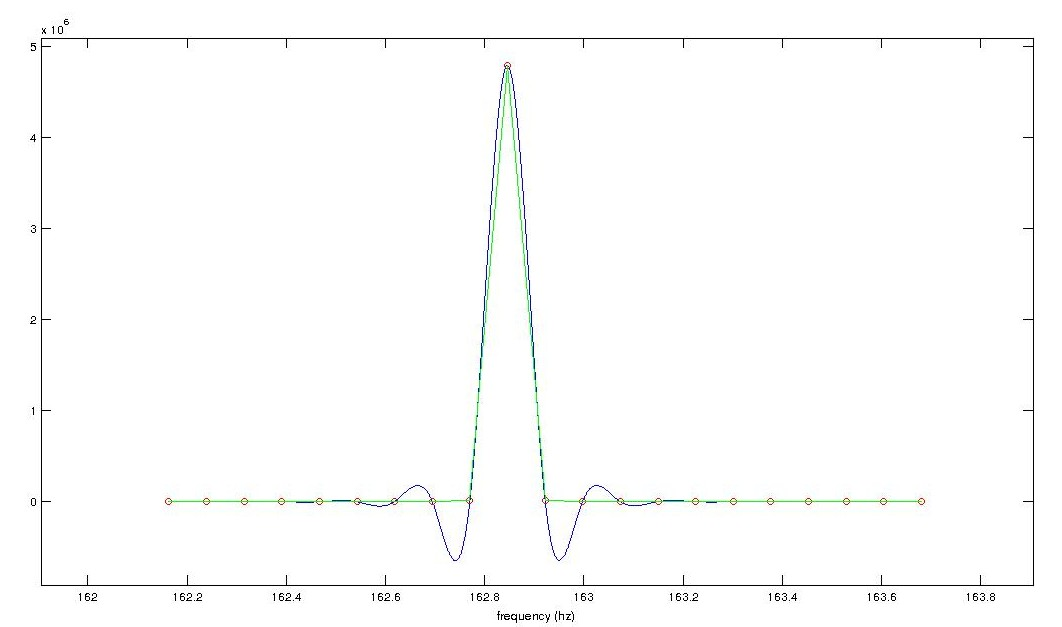
\includegraphics[width=\textwidth*\real{0.9}]{images/ch_05/interpolazione.jpg}
	  \end{center} 
	  \caption{\textit{Interpolazione per migliorare la ricerca del massimo}}  
	  \label{fig:interpolazione}
	\end{figure}

La figura \ref{fig:interpolazione} mostra un esempio dell'interpolazione realizzata. 
I punti evidenziati in rosso, rappresentano il prodotto delle versioni sotto-campionate dello spettro del segnale audio.
La linea verde che li congiunge, rappresenta un'interpolazione lineare.
La linea blu che passa per tutti i punti rappresenta l'interpolazione spline realizzata al fine di trovare il massimo della funzione con una maggiore precisione.

Successivamente all'interpolazione, l'operazione di ricerca del massimo viene effettuata nuovamente e l'ascissa del punto trovato viene utilizzata come frequenza della nota suonata dalla corda della chitarra.

Al fine di eliminare falsi positivi, cioè massimi che possono essere rilevati in momenti in cui non si sta suonando alcuna corda tra quelle della chitarra, è fissata una soglia in ampiezza al di sotto della quale la frequenza del massimo non è ritenuta una frequenza di pitch.
Tramite l'algoritmo \mbox{HPS} è facile distinguere quest'ultimo caso.

In presenza di una nota ad una determinata frequenza, la frequenza fondamentale risulta essere molto amplificata.
Ciò deriva dal prodotto di 5 massimi locali nelle diverse funzioni scalate della trasformata del segnale originale.
Nel caso di rumore, invece, le diverse frequenze pur moltiplicandosi tra loro, non subiscono l'effetto di amplificazione che subisce la frequenza fondamentale nel primo caso.

La soglia minima al di sopra della quale la frequenza viene considerata fondamentale è fissata a 84 dB.
Si ricorda che il segnale su cui è applicata tale soglia, è il risultato della moltiplicazione di cinque segnali, di conseguenza, in presenza di un pitch, il massimo della funzione è sempre al di sopra di tale soglia.


